\documentclass{article}
\usepackage{graphicx}
\usepackage{subcaption}
\usepackage[font=small,labelfont=bf]{caption}
\begin{document}
	
	\title{Data Analysis Results}
	\maketitle
\section*{3 a.m. peak}

If we plot the taxi time averaged over all the flights as a function of the hour of the day we see a peak that cannot be explained by the number of aircraft that are crossing the taxiway (Figure ~\ref{n_avions}).

\begin{figure}[h]
	\centering
	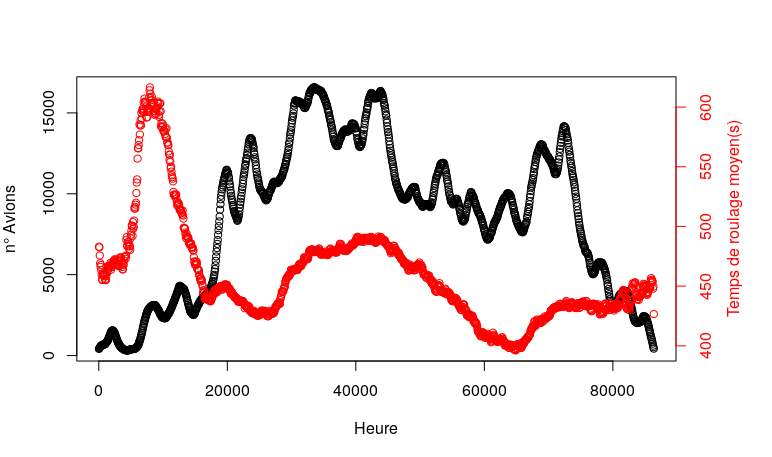
\includegraphics[width=10cm]{n_avions_TempsRoulage}
	\caption{Comparison between number of aircrafts in the taxiway (black line) and taxi time (red line).}
	\label{n_avions}
\end{figure}
	
So we performed an analysis of all the variables that can contribute to the unexplained peak of 3 a.m.

We tested the distance ($d$) between the parking and the runway, the average speed during the taxiing ($v$), the waiting time ($t_w$) of the potential stops of the aircraft during the taxiing (in the middle of the taxiway or at the runway). We chose those variables because we can roughly model the taxi time ($t_t$) as:
\[t_t = \frac{d}{v} + t_w \]

\newpage

	\begin{figure}[h!!!!!!!!!]
		\centering
		\begin{subfigure}[b]{\textwidth}
		\centering
		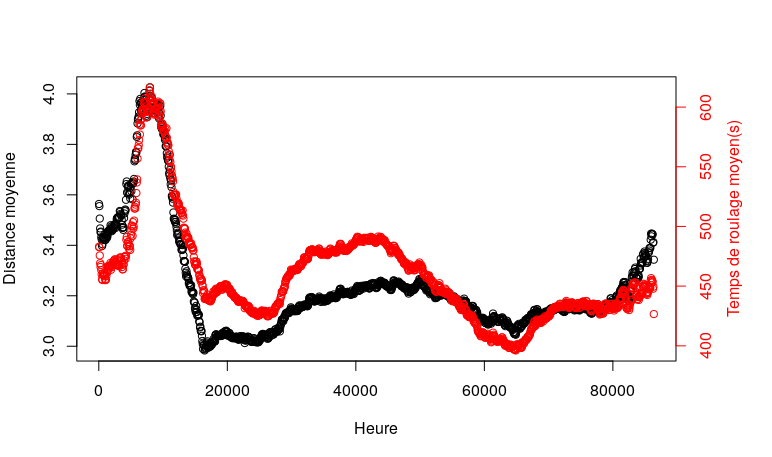
\includegraphics[width=8cm]{Distance_TempsRoulage}
		\caption{Comparison between distance of the parking from the runway (black) and taxi time (red).}
		\label{distance}
		\end{subfigure}
		\begin{subfigure}[b]{\textwidth}
			\centering
		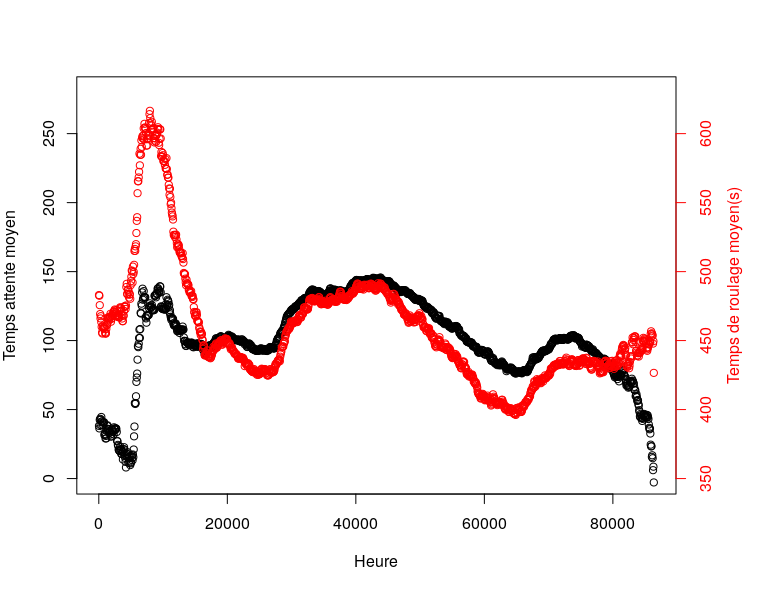
\includegraphics[width=8cm]{temps_attente_TempsRoulage}
		\caption{Comparison between waiting time during the taxiing (black) and taxi time (red).}
		\label{waiting}
		\end{subfigure}
		\begin{subfigure}[b]{\textwidth}
		\centering
		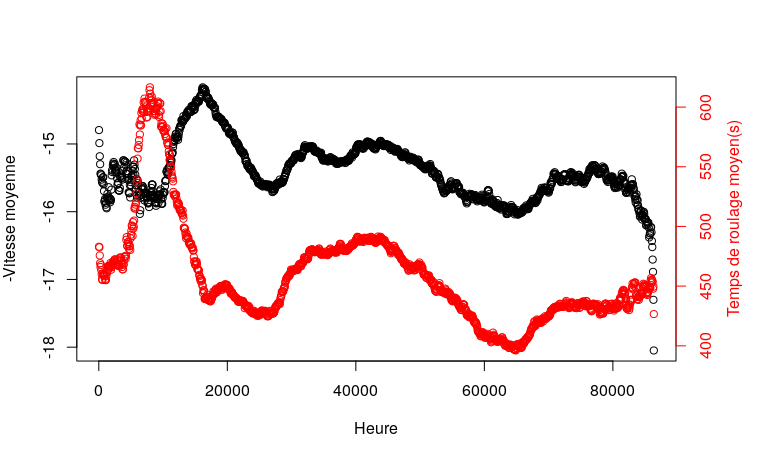
\includegraphics[width=8cm]{vitesse_TempsRoulage}
		\caption{Comparison between the opposite ()since we expect the taxi time to be inversely proportional to the speed) of average speed during the taxiing (black) and taxi time (red).}
		\label{vitesse}
		\end{subfigure}
	\caption{Behavior of average taxi time as a function of the hour of the day compared to the behavior of parking-runway distance, waiting time and speed.}
	\label{comparisons}
	\end{figure}

Figure ~\ref{comparisons} shows the the results.

As we can see from the pictures, what explains better the 3 a.m. peak is the larger distance traveled by the aircrafts on average at that hour. Also the waiting time gives a little contribution, while the speed is on average larger in correspondence of the peak. This means that it gives a negative contribution to the taxi time, with respect to the other hours of the day.

\bigskip
We can go deeper in the analysis of the reasons of a larger taxi time if we hypothesize the dependencies of waiting time, speed and distance from some other variables that we can find in our data set. 

Our first hypothesis about dependencies is the following:

\[d=d(gate,company, number \ of \ aircrafts \ on \ platform, weather)\]
\[v=v(aircraft \ type, weather)\]
\[t_w=t_w(number \ of \ aircrafts \ on \ platform)\]

In fact:
\begin{itemize}
	\item \textit{Distance:} it depends on the company because each company is assigned a terminal or a parking zone, that can be further or closer to the runway (that's why it depends on the gate also). It depends on the number of aircrafts because in case of intense traffic an aircraft parked in the north terminal can leave from the southern runway, if there are less aircrafts waiting there. It depends on the weather because if de-icing procedures are needed, the aircraft necessarily has to pass through de-icing zones.
	\item \textit{Speed:} it depends on the aircraft type because heavier aircrafts are slower on the ground. It de
	pends on the weather because in case of low visibility conditions the pilots must drive slower.
	\item \textit{Waiting time:} it depends on the number of aircrafts in the airport because if there are many aircrafts, the probability of stopping to make another aircraft pass is higher.
 \end{itemize}

For what it concerns the 3 a.m. peak, we looked into the distance dependencies since it's the most influential variable for the taxi time in that time interval. 

We explored the company variable, comparing the frequencies of flights of a specific company at all hours of the day with the ones in the interval from 1:35 a.m. to 3:40 a.m.


\begin{table}[h!!!!!!!!!!!!!!!!]
	\begin{center}
		\caption{Average company frequencies for the whole day (left) and for the time interval 1:35 a.m. - 3.40 a.m. (right)}
		\label{tab:table1}
		\begin{tabular}{l|c} % <-- Alignments: 1st column left, 2nd middle and 3rd right, with vertical lines in between
			\textbf{Company} & \textbf{Frequency}\\
			\hline
			AFR & 48,3\% \\
			EJU & 6,8\% \\
			FDX & 2.25\% \\
		\end{tabular}
	\quad \quad \quad \quad
		\begin{tabular}{l|c} % <-- Alignments: 1st column left, 2nd middle and 3rd right, with vertical lines in between
		\textbf{Company} & \textbf{Frequency}\\
		\hline
		FDX & 26,8\% \\
		AFR & 26,4\% \\
		ABR & 20,3\% \\
		\end{tabular}
	\end{center}
\end{table}

\newpage
We see that in the time interval of interest there are many flights from FedEx and ASL Airlines Ireland (ABR) (that provides for aircrafts to FedEx), in opposition to what happens during the rest of the day, where the flights are mainly from Air France and Easy Jet. 


\end{document}